%versi 2 (8-10-2016)

\chapter{Landasan Teori}
\label{chap:teori}
Pada bab ini dijelaskan dasar-dasar teori mengenai KIRI website, JSON, CSV, dan \textit{Google Maps Javascript API}

\section{KIRI Website }
\label{sec:KIRI} 
KIRI adalah aplikasi navigasi angkutan umum berbasis web yang melayani Bandung dan kota-kota lain di Indonesia.\cite{pascal:17:KIRI}.
Pada awal pembuatannya KIRI dibuat untuk tujuan komersial. Namun karena dinilai kurang sukses projek KIRI sekarang menjadi open source projek yang dapat di akses. Aplikasi KIRI memiliki beberapa fitur sebagai berikut:
\begin{itemize}
	\item Pemilihan rute tercepat menggunakan angkutan kota.
	perangkat lunak KIRI dapat menentukan rute terbaik untuk berpegian dengan angkutan umum. 
	\begin{figure}[H]
	\centering
	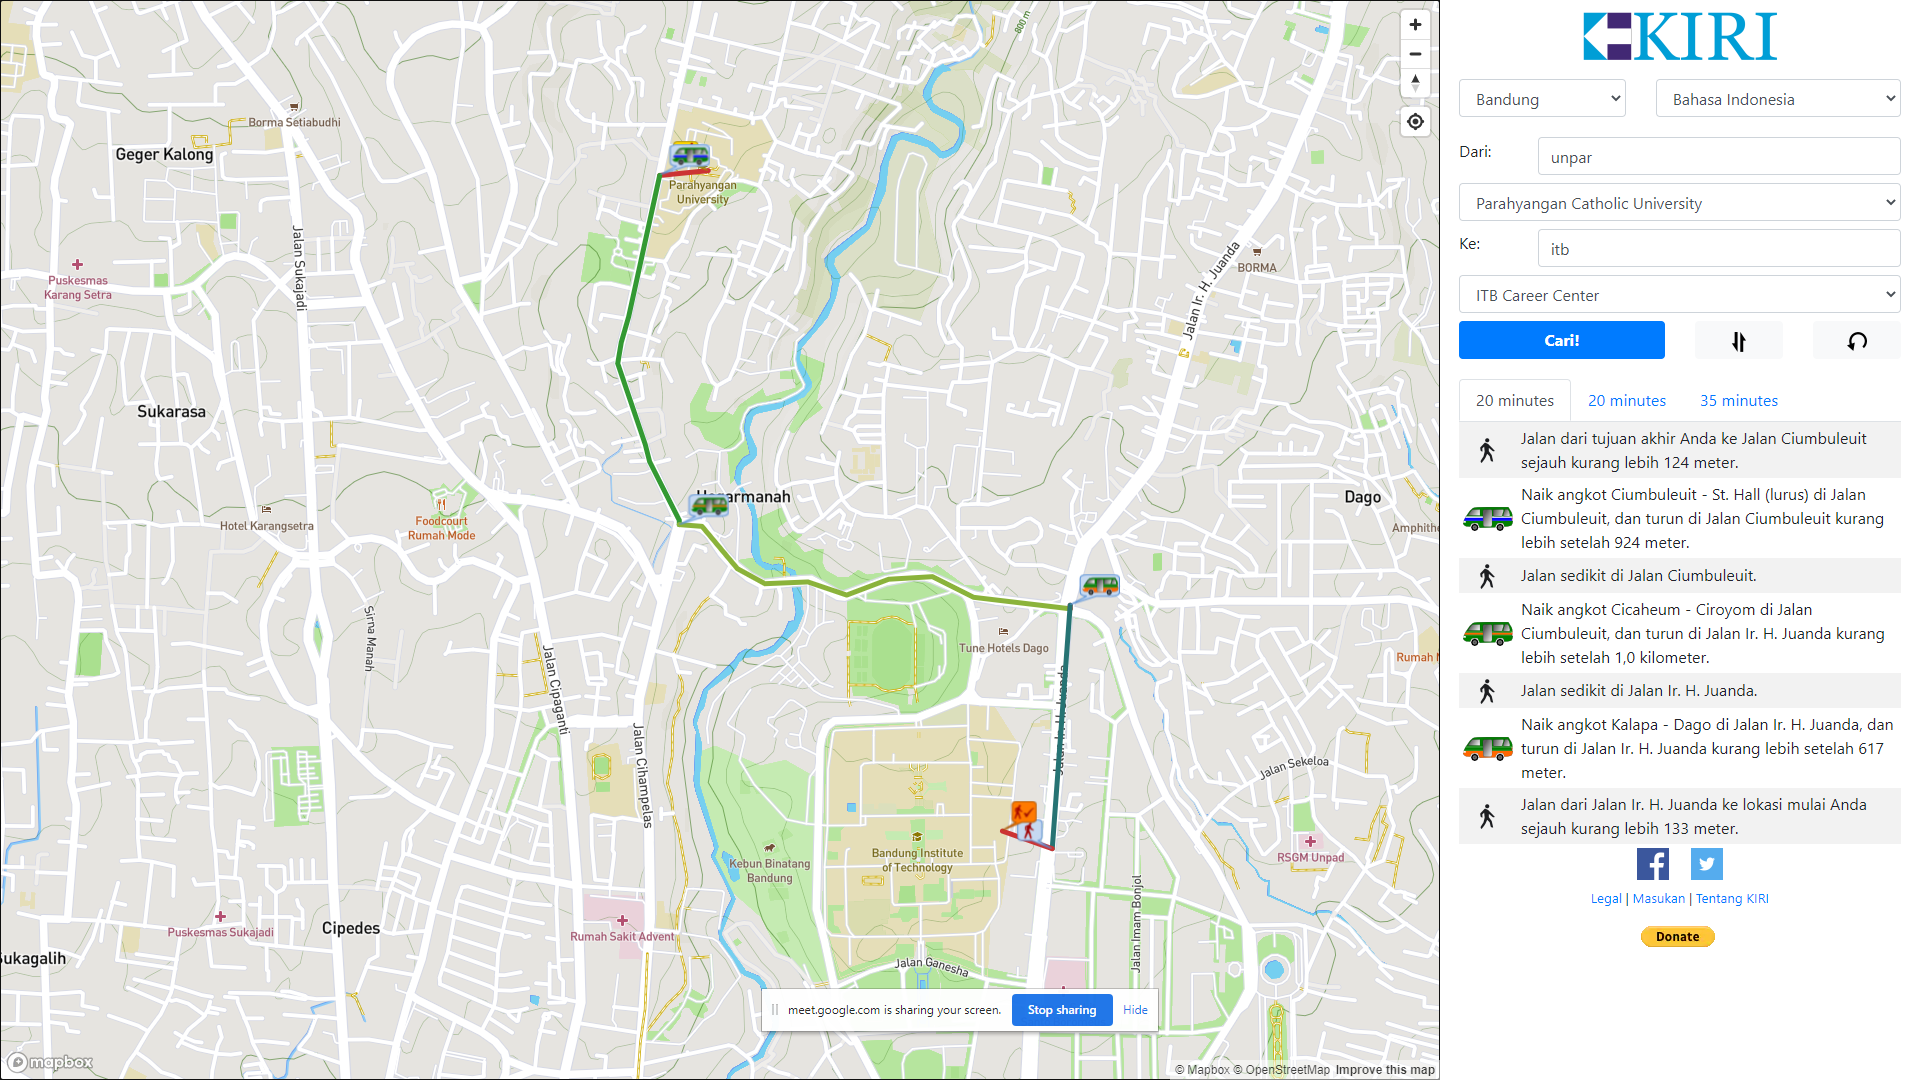
\includegraphics[scale=0.3]{Gambar/kiri-example-1}
	\caption{Tampilan utama website KIRI}
	\label{fig:my_label}
\end{figure}
	\item Memiliki fitur multi bahasa.
	perangkat lunak kiri dilengkapi dengan fitur multi bahasa. 
\begin{figure}[H]
	\centering
	
\includegraphics[scale=0.3]{Gambar/multibahasa.PNG}
	\caption{Multi Bahasa}
	\label{fig:my_label}
\end{figure}
	\item Dapat menampilkan instruksi lengkap  mencapai tujuan.
	perangkat lunak kiri juga menampilkan seluruh instruksi lengkap penggunaan angkutan umum. 
\end{itemize}
\begin{figure}[H]
	\centering
	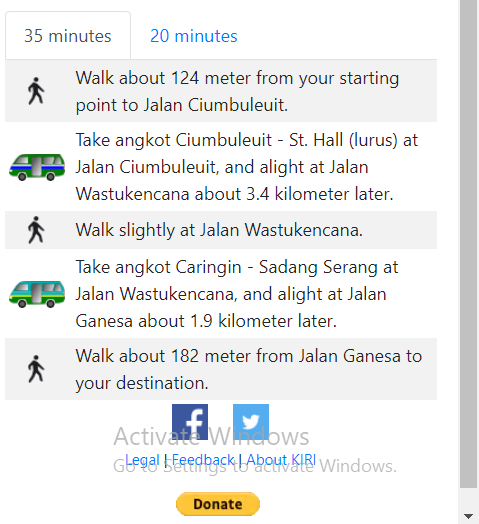
\includegraphics[scale=0.3]{Gambar/instuksi.PNG}
	\caption{Instruksi KIRI}
	\label{fig:my_label}
\end{figure}
 



\section{JSON}
\label{subsec:json}
JSON (\textit{Javascript Object Notation}) adalah format teks untuk melakukan serialisasi data terstruktur\cite{RFC:7159}. JSON berasal objek literal \textit{javascript}, Seperti yang didefinisikan oleh oleh bahasa pemrograman \textit{ECMAScript}, JSON dapat mewakili empat tipe data primitif (\textit{strings}, \textit{numbers}, \textit{booleans}, \textit{null}) dan dua tipe data terstruktur (\textit{objects}, \textit{arrays}).

\subsection{ JSON Grammar}
JSON teks terdiri dari sekumpulan Token. Set Token mencakup enam \textit{structural characters }, \textit{strings}, \textit{numbers} dan tiga nama literal. JSON teks merupakan \textit{serialized value}. JSON membatasi JSON teks menjadi \textit{object} atau \textit{array}. Implementasi JSON hanya boleh menghasilkan \textit{object} atau \textit{array}. JSON memiliki enam \textit{structural characters} yaitu :

\begin{itemize}
	\item \begin{verbatim} begin-array     = ws %x5B ws  ; [ left square bracket. 
	\end{verbatim}
	\item \begin{verbatim} begin-object    = ws %x7B ws  ; { left curly bracket. 
	\end{verbatim}
	\item \begin{verbatim}  end-array       = ws %x5D ws  ; ] right square bracket. 
	\end{verbatim}
	\item \begin{verbatim}  end-object      = ws %x7D ws  ; } right curly bracket. 
	\end{verbatim}
	\item \begin{verbatim}  name-separator  = ws %x3A ws  ; : colon.
	\end{verbatim}
	\item \begin{verbatim}  value-separator = ws %x2C ws  ; , comma.
	\end{verbatim}
\end{itemize}
Penggunaan \textit{whitepace} sebelum atau setelah enam \textit{structural characters} diperbolehkan.
\begin{verbatim} 
 ws = *(
              %x20 /              ; Space
              %x09 /              ; Horizontal tab
              %x0A /              ; Line feed or New line
              %x0D )              ; Carriage return
\end{verbatim}
    
\subsection{Values}
\textit{JSON value} harus berupa \textit{object}, \textit{array}, \textit{number}, atau \textit{string}, atau salah satu dari tiga \textit{literal names}:
\begin{itemize}
	\item true.
	\item false.
	\item null.
\end{itemize}
Setiap \textit{literal names} harus tersusun dari huruf kecil. Selain  \textit{literal names} yang disebutkan diatas tidak ada \textit{literals names} lain yang izinkan.

\begin{lstlisting}
      value = false / null / true / object / array / number / string

      false = %x66.61.6c.73.65   ; false

      null  = %x6e.75.6c.6c      ; null

      true  = %x74.72.75.65      ; true
\end{lstlisting}

\subsection{Objects}
\textit{Object} direpresentasikan dengan sepasang kurung kurawal ({}) kosong atau berisi name/\textit{value pair} atau (\textit{members)}. Nama pada \textit{objects} berupa \textit{string}. Setelah nama akan dikuti oleh simbol \textit{colon (:)} yang berfungsi untuk memisahkan nama dengan \textit{value}. Setelah value akan diikuti dengan simbol koma (,). Nama pada \textit{Object} harus bersifat unik.

\begin{lstlisting}
      object = begin-object [ member *( value-separator member ) ]
               end-object

      member = string name-separator value
\end{lstlisting}
\textit{Object} dengan susunan nama yang unik akan dapat beroperasi dan diimplementasikan oleh semua software. Jika susunan nama pada \textit{object} tidak bersifat unik maka respon perangkat lunak yang menerima \textit{object} tersebut tidak dapat diprediksi.

\subsection{Arrays}
\textit{Arrays} direpresentasikan dengan sepasang kurung siku ([]) kosong atau berisi satu atau lebih element. Elements pada array akan dipisahkan dengan simbol koma (,).

\begin{lstlisting}
    array = begin-array [ value *( value-separator value ) ] end-array
\end{lstlisting}
Tidak ada persyaratan bahwa \textit{value} pada array harus memiliki tipe data yang sama.

\subsection{Numbers}
\textit{Numbers} direpresentasikan menggunakan basis 10 \textit{decimal}, \textit{Number} bisa memiliki \textit{prefix} seperti simbol minus (-), \textit{Number} juga biasanya dilengkapi dengan pecahan dan eksponen. Dalam penulisan \textit{number} \textit{leading zero} tidak diperbolehkan. \textit{Pecahan} adalah \textit{decimal point} yang diikuti oleh satu atau lebih digit. \textit{Eksponen} biasanya diawali dengan \textit{character} E yang bisa diikuti dengan simbol opsional \textit{plus} atau \textit{minus}. Huruf E dan simbol opsional akan diikuti oleh satu atau lebih digit.
Nilai \textit{Numeric} yang tidak diperbolehkan dalam aturan penulisan dibawah seperti (\textit{NaN} dan \textit{Infinity}).

\begin{lstlisting}
        number = [ minus ] int [ frac ] [ exp ]

      decimal-point = %x2E       ; .

      digit1-9 = %x31-39         ; 1-9

      e = %x65 / %x45            ; e E

      exp = e [ minus / plus ] 1*DIGIT

      frac = decimal-point 1*DIGIT

      int = zero / ( digit1-9 *DIGIT )

      minus = %x2D               ; -

      plus = %x2B                ; +

      zero = %x30                ; 0
\end{lstlisting}
Spesifikasi ini memungkinkan implementasi untuk menetapkan batasan pada rentan  dan ketepatan angka yang diterima. Sejak banyak \textit{software} mengimplementasikan \textit{ IEEE 754-2008 binary64 (double precision) numbers}, Untuk mendapatkan performa yang baik maka \textit{implementasi} tidak boleh melebihi \textit{precision} atau \textit{range} yang disediakan.

\subsection{Strings}
\textit{String} direpresentasikan dengan simbol \textit{quotation marks} semua \textit{unicode} akan diletakan diantara simbol \textit{quotation marks}, Kecuali beberapa \textit{character} yang khusus yang harus melalui proses \textit{escape}:
\begin{itemize}
    \item Quotation mark.
    \item Reverse solidus.
    \item Control characters \textit{(U+0000,U+001F).} .
\end{itemize}
Untuk melakukan \textit{escape} pada \textit{extended character} atau pada \textit{character} yang tidak dalam bentuk penulisan standart, \textit{character} dapat direpresentasikan kedalam \textit{12-character sequence}.

\begin{lstlisting}
      string = quotation-mark *char quotation-mark

      char = unescaped /
          escape (
              %x22 /          ; "    quotation mark  U+0022
              %x5C /          ; \    reverse solidus U+005C
              %x2F /          ; /    solidus         U+002F
              %x62 /          ; b    backspace       U+0008
              %x66 /          ; f    form feed       U+000C
              %x6E /          ; n    line feed       U+000A
              %x72 /          ; r    carriage return U+000D
              %x74 /          ; t    tab             U+0009
              %x75 4HEXDIG )  ; uXXXX                U+XXXX

      escape = %x5C              ; \

      quotation-mark = %x22      ; "

      unescaped = %x20-21 / %x23-5B / %x5D-10FFFF
\end{lstlisting}

\subsection{JSON Example}
Berikut ini adalah contoh penulisan \textit{JSON}
\begin{itemize}
    \item Contoh  JSON Object
    \begin{lstlisting}
        {
        "Image": {
            "Width":  800,
            "Height": 600,
            "Title":  "View from 15th Floor",
            "Thumbnail": {
                "Url":    "http://www.example.com/image/481989943",
                "Height": 125,
                "Width":  100
            },
            "Animated" : false,
            "IDs": [116, 943, 234, 38793]
          }
      }
    \end{lstlisting}
    \textit{Image member} adalah sebuah \textit{object} yang memiliki \textit{Thumbnail member} yang merupakan sebuah  \textit{object} dan \textit{IDs Member} yang merupakan sebuah \textit{array}.
    
    \item Contoh JSON \textit{Array} dengan dua buah \textit{elements} yang berupa \textit{object} 
        \begin{lstlisting}
     [
        {
           "precision": "zip",
           "Latitude":  37.7668,
           "Longitude": -122.3959,
           "Address":   "",
           "City":      "SAN FRANCISCO",
           "State":     "CA",
           "Zip":       "94107",
           "Country":   "US"
        },
        {
           "precision": "zip",
           "Latitude":  37.371991,
           "Longitude": -122.026020,
           "Address":   "",
           "City":      "SUNNYVALE",
           "State":     "CA",
           "Zip":       "94085",
           "Country":   "US"
        }
      ]

    \end{lstlisting}
    \item Contoh JSON teks yang hanya memiliki \textit{values} 
    \begin{lstlisting}
    "hello world"
    32 
    false
    \end{lstlisting}
\end{itemize}
   
\section{CSV}
\label{subsec:csv}
CSV (\textit{Comma Separated Values}) adalah format penyajian data yang sudah umum digunakan dibanyak progam \textit{spreadsheet}, CSV memiliki format memisahkan setiap value dengan simbol titik koma (;) dan menggunakan baris baru sebagai penanda pemisah antar element data\cite{RFC:4180}.

\subsection{CSV Format}
Tidak ada spesifikasi \textit{formal} dalam penulisan csv. Format csv yang akan dituliskan pada dokumen ini adalah format yang paling banyak diimplementasikan:

\begin{itemize}
    \item Setiap field diletakan pada baris terpisah dan dipisahkan oleh \textit{line break (CLRF)} contoh:
    \begin{lstlisting}
          aaa,bbb,ccc CRLF
          zzz,yyy,xxx CRLF
    \end{lstlisting}
    \item \textit{Field} terakhir pada format csv tidak harus menggunakan \textit{line break (CLRF)} contoh:
        \begin{lstlisting}
          aaa,bbb,ccc CRLF
          zzz,yyy,xxx 
    \end{lstlisting}
    \item Memungkinkan adanya eksternal \textit{header} yang memiliki aturan penulisan yang sama dengan element pada csv. Nilai pada eksternal \textit{header} akan mewakili nama yang tercantum pada \textit{field} jumlah eksternal \textit{header} harus sama dengan jumlah kolom pada normal record contoh:
    \begin{lstlisting}
       field_name,field_name,field_name CRLF
       aaa,bbb,ccc CRLF
       zzz,yyy,xxx CRLF

    \end{lstlisting}
    
    \item Memungkinkan ada satu atau lebih, \textit{field} yang dipisahkab oleh koma (,). Setiap baris harus memiliki jumlah \textit{field} yang sama pada satu \textit{file}. Spasi dianggap sebuah element pada \textit{field} yang tidak dapat diabaikan. Pada field terkahir sebuah baris tidak boleh diberikan simbol koma (,) contoh:
    \begin{lstlisting}
       aaa,bbb,ccc
    \end{lstlisting}
    
    \item Setiap \textit{Field} bisa menggunakan simbol \textit{double quotes}. Jika \textit{field} tidak menggunakan simbol \textit{double quotes} maka \textit{double quotes} tidak akan ditampilkan pada \textit{fields}
    \begin{lstlisting}
      "aaa","bbb","ccc" CRLF
       zzz,yyy,xxx
    \end{lstlisting}
    
    \item Jika simbol \textit{double quotes} meruapakan salah satu elemn pada \textit{field}, Maka simbol \textit{double quotes} tersebut harus diescape dengan memberikan simbol \textit{double quotes} lain didalam \textit{field} tersebut contoh:
    \begin{lstlisting}
      "aaa","b""bb","ccc"
    \end{lstlisting}
\end{itemize}

% Beberapa istilah dalam \textit{CSV} berdasarkan \textit{ABNF Grammar} :
% \begin{lstlisting}

%   file = [header CRLF] record *(CRLF record) [CRLF]

%   header = name *(COMMA name)

%   record = field *(COMMA field)

%   name = field

%   field = (escaped / non-escaped)

%   escaped = DQUOTE *(TEXTDATA / COMMA / CR / LF / 2DQUOTE) DQUOTE

%   non-escaped = *TEXTDATA

%   COMMA = %x2C

%   CR = %x0D ;as per section 6.1 of RFC 2234 [2]
%       DQUOTE =  %x22 ;as per section 6.1 of RFC 2234 [2]

%   LF = %x0A ;as per section 6.1 of RFC 2234 [2]

%   CRLF = CR LF ;as per section 6.1 of RFC 2234 [2]

%   TEXTDATA =  %x20-21 / %x23-2B / %x2D-7E
% \end{lstlisting}


\section{Node.js}
\textit{Node.js} merupakan \textit{asynchronous event-driven JavaScript runtime}. Dengan menggunakan Node.js memungkinkan untuk menjalankan perintah \textit{javascript} tanpa menggunakan \textit{web browser}, \textit{Node.js} memungkinkan untuk menjalankan dan melakukan \textit{server-side scripting}\cite{Nodejs:01:about}. \textit{Node.js} didesain untuk membuat \textit{network applications} yang \textit{scaleable}. Berikut ini contoh syntax \textit{Node.js}:

\begin{lstlisting}
const http = require('http');

const hostname = '127.0.0.1';
const port = 3000;

const server = http.createServer((req, res) => {
  res.statusCode = 200;
  res.setHeader('Content-Type', 'text/plain');
  res.end('Hello World');
});

server.listen(port, hostname, () => {
  console.log(`Server running at http://${hostname}:${port}/`);
});
\end{lstlisting}


\subsection{Struktur File Node.js Project}
	Pada saat membuat projek baru, Node.js membuat \textit{file-file} dasar secara otomatis. \textit{File-file} tersebut memiliki fungsi tersendiri. Folder \textit{node\_modules} berfungsi sebagai penyimpanan semua \textit{library} yang diinstal melalui npm. Semua \textit{library} yang diinstall melalui npm akan dicatat pada file \textit{package.json}, Hal ini bertujuan untuk mempermudah proses \textit{maintence library} pada projek \textit{node.js}.
	
	Struktur dari \textit{file-file} akan berbentuk seperti:
        	\dirtree{%
        .1 root.
        .2 node\_modules.
        .3 \hyperref[dir1-file1]{''file1''}.
        .3 \hyperref[dir1-file2]{''file2''}.
        .2 package.json.
        }


\subsection{\textit{Node Package Manager}}
\textit{Node Package Manager}(NPM) adalah \textit{software registry} yang dimiliki oleh \textit{Node.js}, NPM memungkinkan pengguna untuk mempublikasi atau menggunakan \textit{software library}\cite{npmjs:01:about}. NPM terdiri dari tiga komponen penting yaitu:
\begin{itemize}
    \item NPM website.
    \item NPM CLI ( \textit{Command Line Interface}). 
    \item NPM \textit{Registry}.
\end{itemize}
NPM memiliki beberapa kegunaan antara lain:

\begin{itemize}
    \item Mendownload \textit{Software Library}.
    \item Menjalankan \textit{packages} tanpa harus mendownload \textit{npx}.
    \item Mempublikasikan \textit{Tools} atau \textit{Software Library}.
\end{itemize}

\subsection{NPM CLI}
\textit{NPM} akan terinstall secara otomatis pada perangkat keras ketika menambahkan node.js. Untuk mempermudah proses pembuatan perangkat lunak, Penggunaan \textit{Command Line Interface} (CLI) akan menjadi salah satu \textit{point} penting. NPM memiliki tiga komponen utama dalam penulisan perintah CLI, Komponen ini akan berbentuk seperti:
\begin{verbatim}
    npm <command> [args]
\end{verbatim}
\textit {NPM CLI} memiliki perintah-perintah yang dapat digunakan untuk membantu melakukan \textit{maintenance} terhadap \textit{library} pada projek \textit{node.js}. Berikut perintah-perintah pada \textit{npm cli}:

\begin{itemize}
    \item Command untuk menginisialisasi \textit{npm package} file dapat menggunakan perintah:
    \begin{lstlisting}
      npm init [--force|-f|--yes|-y|--scope]
      npm init <@scope> (same as `npx <@scope>/create`)
      npm init [<@scope>/]<name> (same as `npx [<@scope>/]create-<name>`)
    \end{lstlisting}
    \item Command untuk menambahkan \textit{package} / \textit{library} dapat menggunakan perintah:
    \begin{lstlisting}
        npm install (with no args, in package dir)
        npm install [<@scope>/]<name>
        npm install [<@scope>/]<name>@<tag>
        npm install [<@scope>/]<name>@<version>
        npm install [<@scope>/]<name>@<version range>
        npm install <alias>@npm:<name>
        npm install <git-host>:<git-user>/<repo-name>
        npm install <git repo url>
        npm install <tarball file>
        npm install <tarball url>
        npm install <folder>
    \end{lstlisting}
    \item Command untuk menghapus \textit{package} / \textit{library} dapat menggunakan perintah:
    \begin{lstlisting}
        npm uninstall [<@scope>/]<pkg>[@<version>]
        
    \end{lstlisting}
    % \item Command untuk mempublikasian \textit{package} / \textit{library} dapat menggunakan perintah:
    % \begin{lstlisting}
    % npm publish [<tarball>|<folder>] [--tag <tag>] [--access <public|restricted>] [--otp otpcode] [--dry-run]
    % Publishes '.' if no argument supplied
    % Sets tag 'latest' if no --tag specified
    % \end{lstlisting}
    
\end{itemize}


\section{\textit{Expressjs}}
\textit{Express.js} merupakan \textit{web application framework} untuk \textit{node.js}. \textit{Express.js} menyediakan \textit{robust feature} dalam pembuatan  perangkat lunak berbentuk situs web maupun perangkat begerak\cite{expressjs:01:about}. 

\subsection{Instalasi}
\textit{Express.js} dapat diinstal dengan menggunakan npm. Untuk menambahkan \textit{package express.js} dapat menggunakan perintah:
\begin{verbatim}
    npm install express --save
\end{verbatim}
Ketika menjalankan perintah diatas maka secara otomatis akan menambahkan \textit{library express.js} yang akan disimpan pada \textit{folder} \textit{package.json}.

\subsection{Struktur File Express.js}
\textit{Express.js} tidak memberikan aturan baku dalam penyusunan struktur file dalam pengembangan perangkat lunak. namun \textit{express.js} menyediakan \textit{application generator} yang disebut \textit{express generator} untuk mempermudah pihak pengembang dalam pembuatan perangkat lunak\cite{expressjs:01:about}. Untuk dapat menggunakan \textit{express generator} pengembang harus menambahkan \textit{library} \textit{express generator} melalui npm dengan menggunakan perintah:

\begin{verbatim}
    npx express-generator
\end{verbatim}
Secara otomatis \textit{express} akan menghasilkan sebuah folder yang memiliki struktur file seperti:
    	\dirtree{%
        .1 app.js.
        .2 bin.
        .3 \hyperref[dir1-file1]{www}.
        .2 package.json.
        .2 public.
        .3 \hyperref[dir1-file1]{images}.
        .3 \hyperref[dir1-file1]{javascripts}.
        .3 \hyperref[dir1-file1]{stylesheets}.
        .2 routes.
        .3 \hyperref[dir1-file1]{index.js}.
        .3 \hyperref[dir1-file1]{users.js}.
        .2 views.
        .3 \hyperref[dir1-file1]{index.pug}.
        .3 \hyperref[dir1-file1]{error.pug}.
        .3 \hyperref[dir1-file1]{layout.pug}.
        }
        

\subsection{Routing}
\textit{Routing} adalah proses untuk menentukan cara perangkat lunak merespon \textit{input} melalui beberapa \textit{endpoint}. Dalam pembuatan \textit{routing} pada \textit{express.js} terdapat empat komponen penting yaitu:
\begin{itemize}
    \item Instansi dari \textit{express.js} (app).
    \item \textit{Method} \textit{http method}.
    \item \textit{Path}
    \item Perintah yang akan dijalankan jika \textit{route} dijalankan \textit{Handler}.
\end{itemize}
Pembuatan \textit{routing} pada \textit{express.js} memiliki struktur perintah sebagai berikut:
\begin{verbatim}
    app.METHOD(PATH, HANDLER)
\end{verbatim}
Berikut ini beberapa contoh perintah pembuatan \textit{route} pada \textit{express.js}
\begin{lstlisting}
    app.get('/', function (req, res) {
      res.send('Hello World!')
    })
    
    app.post('/', function (req, res) {
      res.send('Got a POST request')
    })
    
    app.put('/user', function (req, res) {
      res.send('Got a PUT request at /user')
    })
    
    app.delete('/user', function (req, res) {
      res.send('Got a DELETE request at /user')
    })
\end{lstlisting}

\subsection{Menampilkan File Statis}
Untuk dapat menampilkan \textit{file} yang bersifat statis seperti foto, \textit{javascript}, dan \textit{css}, \textit{express.js} telah menyediakan objek \begin{verbatim}
    express.static(root, [options])
\end{verbatim}[] 
Parameter \textit{root} menandakan \textit{root directory} untuk menampilkan \textit{file} statis. Contoh perintah untuk menampilkan \textit{file} statis:

\begin{lstlisting}
app.use('/static', express.static('public'))
\end{lstlisting}
Parameter '/static' berutujuan untuk membuat \textit{virtual path} yang memiliki \textit{prefix}  '/static', sedangkan parameter'public' menandakan bahwa \textit{file} statis berada didalam \textit{folder public}. Perintah diatas ketika dijalankan maka \textit{express} akan secara otomatis membuat \textit{route} seperti:
\begin{lstlisting}
http://localhost:3000/static/images/kitten.jpg
http://localhost:3000/static/css/style.css
http://localhost:3000/static/js/app.js
http://localhost:3000/static/images/bg.png
http://localhost:3000/static/hello.html
\end{lstlisting}
yang dapat digunakan untuk mengakses \textit{file} statis.

	
\section{Google Maps Javascript API}
\label{sec:googlemaps}
Pada subbab ini akan menjelaskan tentang \textit{google maps javascript api} beserta kelas-kelas yang dimilikinya. Google Maps adalah layanan pemetaan web yang dikembangkan oleh Google. Menawarkan citra satelit, foto udara, dan peta jalan yang interaktif, kondisi lalu lintas secara \textit{real time}. Dalam pengembangannya \textit{google maps} memiliki akses pendukung untuk bahasa pemrograman \textit{javascript}. Berikut ini beberapa layanan yang telah disediakan oleh \textit{google maps javascript api\cite{googlemaps:01:refrence}}:

\begin{itemize}
    \item \textit{Maps}.
    \item \textit{Drawing Object}.
    \item \textit{Street Views}.
    \item \textit{Routes}
\end{itemize}

\subsection{Map}
\textit{Map} adalah sebuah objek pada \textit{google maps javascript api} yang digunakan untuk membuat objek \textit{map} didalam \textit{html} elemen. Untuk dapat menginisialisasi objek \textit{map} pengembang harus dapat menggunakan constructor yang memiliki perintah:
\begin{lstlisting}
    Map(mapDiv[, opts])
    Parameters: 
    mapDiv:  Element
    opts:  MapOptions optional
\end{lstlisting}
Pada \textit{constructor} diatas terdapat dua paramete:
\begin{itemize}
    \item mapDiv.
    \item MapOptions
\end{itemize}
\textit{MapDiv} adalah elemen html dimana objek map akan diinisialisasi, parameter ini bersifat wajib. MapOptions adalah sebuah objek yang dapat digunakan untuk mengatur \textit{property} yang dimiliki oleh objek \textit{map}. Berikut ini adalah contoh menginisialisasi objek \textit{map}:
\begin{lstlisting}
    function initMap() {
        let mapOptions = {
            center: {lat: -6.914744, lng: 107.609810},
            zoom: 12,
    }
    let map = new google.maps.Map(document.getElementById("map"), mapOptions);
    return map;
    }
\end{lstlisting}
Ketika fungsi \textit{initMap()} dijalankan maka \textit{google maps javascript api} akan membuat objek map didalam \textit{html dom} yang memiliki id='map' dan akan mengatur \textit{property} yang dimiliki sesuai dengan objek \textit{mapOptions}.

Objek \textit{map} telah menyediakan fungsi-fungsi yang bisa langsung digunakan oleh pengembang, beberapa fungsi yang disediakan oleh  objek \textit{map} adalah:

\begin{itemize}
    \item Fungsi \textit{fitBounds}  berguna untuk menentukan \textit{view port} dari objek \textit{map} sesuai dengan \textit{bounds} yang diberikan. Fungsi ini memiliki struktur perintah seperti:
    \begin{lstlisting}
        fitBounds(bounds[, padding])
        Parameters: 
        bounds:  LatLngBounds|LatLngBoundsLiteral
        padding:  number|Padding optional
        Return Value:  None
    \end{lstlisting}
    \item Fungsi \textit{getBounds}  berguna untuk mendapatkan \textit{view port} dari objek \textit{map}. Fungsi ini memiliki struktur perintah seperti:
    \begin{lstlisting}
        getBounds()
        Parameters:  None
        Return Value:  LatLngBounds
    \end{lstlisting}
    \item Fungsi \textit{getCenter}  berguna untuk mendapatkan posisi yang ditunjukan pada objek \textit{map} posisi yang didapatkan akan berbentuk \textit{longtitude dan langtitude}. Fungsi ini memiliki struktur perintah seperti:
    \begin{lstlisting}
        getCenter()
        Parameters:  None
        Return Value:  LatLng
    \end{lstlisting}
    \item Fungsi \textit{getClickableIcons} berguna untuk mendapatkan \textit{clickable icon} setiap \textit{clickable icon} merupakan \textit{point of interest} pada \textit{map} . Fungsi ini memiliki struktur perintah seperti:
    \begin{lstlisting}
        getClickableIcons()
        Parameters:  None
        Return Value:  boolean
    \end{lstlisting}
    \item Fungsi \textit{getMapTypeId} beguna untuk mendapatkan \textit{id} dari jenis \textit{map} yang digunakan . Fungsi ini memiliki struktur perintah seperti:
    \begin{lstlisting}
        getMapTypeId()
        Parameters:  None
        Return Value:  MapTypeId|string
    \end{lstlisting}
    \textit{Google Maps Javascript API} menyediakan variabel konsanta / \textit{constant} yang berfungsi untuk menentukan jenis peta yang akan digunakan pada objek \textit{map}. Konsanta ini dapat memiliki empat nilai yaitu:
    \begin{itemize}
        \item HYBRID jenis peta ini akan menampilkan layar \textit{transparan} pada jalan-jalan utama pada citra satelit.
        \item ROADMAP jenis peta ini akan menampilkan \textit{street map}.
        \item SATELLITE jenis peta ini akan menampilkan citra satellite.
        \item TERRAIN jenis peta ini akan menampilkan bentuk nyata dari kondisi geologi suatu tempat.
    \end{itemize}
    \item Fungsi \textit{setMapTypeId} beguna untuk membuat atau mengubah \textit{mapTypeId}. Fungsi ini memiliki struktur perintah seperti:
    \begin{lstlisting}
        setMapTypeId(mapTypeId)
        Parameters: 
        mapTypeId:  MapTypeId|string
    \end{lstlisting}
    \item Fungsi \textit{setZoom} berguna untuk mengubah \textit{zoom  value} yang dimiliki oleh objek \textit{map}.
    \begin{lstlisting}
        setZoom(zoom)
        Parameters: 
        zoom:  number
    \end{lstlisting}
    \item Fungsi \textit{setMapOption} berguna untuk mengubah \textit{property mapOption} yang dimiliki oleh objek \textit{map}.
    \begin{lstlisting}
    setOptions(options)
    Parameters: 
    options:  MapOptions
    \end{lstlisting}
\end{itemize}

\subsection{Sistem Kordinat  Google Maps}
\textit{Google Maps Javascript API} menggunakan  kelas \textit{LatLng} untuk merepresentasikan kordinat secara geografis pada objek \textit{map}. Kelas \textit{LatLng} merupakan sebuah kelas yang merepresentasikan latitude dan longtitude
\begin{itemize}
    \item Latitude memiliki batas antara -90 sampai 90 derajat, jika ada nilai yang diluar batasan tersebut maka nilai tersebut akan dibulatkan kebatas terdekat.
    \item Longtitude memiliki batas antara -180 sampai 180 derajat, jika ada nilai yang diluar batasan tersebut maka nilai tersebut akan dibulatkan kebatas terdekat. 
\end{itemize}

Untuk dapat menginisialisasi kelas \textit{LatLng} pada \textit{google maps javascript api} pengembang perlu membuat \textit{constructor} yang memiliki struktur:
\begin{lstlisting}
    LatLng(lat, lng[, noWrap])
    Parameters: 
    lat:  number
    lng:  number
    noWrap:  boolean optional
\end{lstlisting}
Membuat objek LatLng yang mewakili titik geografis. \textit{latitude} ditentukan dalam derajat dalam rentang [-90, 90]. \textit{longtitude} ditentukan dalam derajat dalam rentang [-180, 180]. Set \textit{noWrap} \textit{true}  untuk mengaktifkan nilai di luar rentang ini. Contoh penggunaan kelas \textit{LatLng}:
\begin{lstlisting}
     map.setCenter(new google.maps.LatLng(-34, 151));
     map.setCenter({lat: -34, lng: 151}); 
\end{lstlisting}
\textit{Google Maps Javascript API} telah menyediakan fungsi bawaan yang dapat diakses ketika menggunakan kelas \textit{LatLng}. Fungsi tersebut adalah:
\begin{itemize}
    \item Fungsi \textit{equals} fungsi ini bertujuan untuk membandingkan posisi antara objek \textit{map}.
    \begin{lstlisting}
         equals(other)
         Parameters: 
         other:  LatLng
         Return Value:  boolean
    \end{lstlisting}
    \item Fungsi \textit{lat} fungsi ini bertujuan untuk mendapatkan posisi \textit{latitude} dari  objek \textit{map}.
    \begin{lstlisting}
        lat()
        Parameters:  None
        Return Value:  number
        Returns the latitude in degrees.
    \end{lstlisting}
    \item Fungsi \textit{lng} fungsi ini bertujuan untuk mendapatkan posisi \textit{longtitude} dari  objek \textit{map}.
    \begin{lstlisting}
        lng()
        Parameters:  None
        Return Value:  number
        Returns the longitude in degrees.
    \end{lstlisting}
    \item Fungsi \textit{toJSON} fungsi ini akan mengembalikan format \textit{json} terhadap posisi latlng padda objek \textit{map}
    \item Fungsi \textit{toUrlValue} Mengembalikan string dalam bentuk "lat, lng" untuk LatLng ini.
\end{itemize}
\subsection{Drawing System}
Pada subbab ini akan dijelaskan cara penggunaan kelas \textit{overlay} yang disediakan oleh \textit{google maps javascript api}. \textit{Google Maps Javascript API } memiliki  kelas-kelas yang digunakan untuk menggambar suatu objek didalam objek \textit{map}. Beberapa kelas \textit{overlay} yang disediakan adalah sebagai berikut:

\begin{itemize}
    \item \textit{Marker}.
    \item \textit{Heat Map}.
\end{itemize}

\subsection{Marker}
\label{sec:mark}
  \begin{figure}[H]
    \centering
    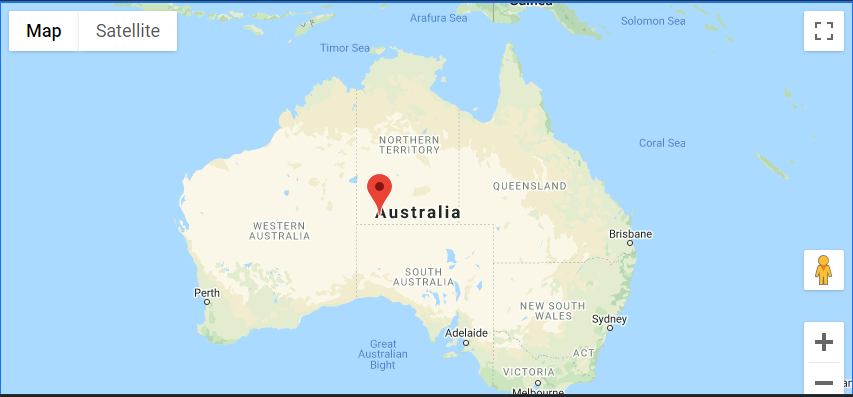
\includegraphics[scale=0.5]{Gambar/add_marker.PNG}
    \caption{Add Marker}
    \label{fig:my_label}
\end{figure}

\textit{Marker} adalah sebuah kelas yang dapat memunculkan \textit{mark} / tanda pada objek \textit{map}. Untuk dapat menginisilasisasi kelas \textit{marker} pengembang dapat menggunakan \textit{constructor} yang memiliki struktur seperti:
\begin{lstlisting}
    Marker([opts])
    Parameters: 
    opts:  MarkerOptions optional
\end{lstlisting}
Pada \textit{constructor} \textit{marker} terdapat parameter \textit{markeroptions} yang bersifat optional. \textit{MarkerOptions} merupakan sebuah objek yang dapat digunakan pada objek \textit{mark}. \textit{MarkerOptions} memiliki properti yang dapat digunakan  seperti:

\begin{table}[H] 
	\centering 
	\caption{Tabel Properti Pada Objek Marker}
	\label{tab:radioPackages}
	\begin{tabular}{|p{8cm}|p{8cm}|}
	\hline
		Properi & Deksripsi \\
    \hline
    	Properti \textit{anchorPoint}.& Nilai offset dari objek marker terhadap info window. \\
    	Properti \textit{animation}.  & Animasi yang akan digunakan ketika objek marker diinisialisasikan.  \\
    	Properti \textit{clickable}.  & Properti penanda jika objek marker diklik.  \\
    	Properti \textit{crossOnDrag}.  & Properti penanda jika objek marker didrag oleh pengguna. \\
    	Properti \textit{cursor}.  & Properti yang akan menunjukan \textit{cursor}  ketika objek marker di \textit{hover}. \\
    	Properti \textit{dragable}.  & Properti bertipe \textit{boolean} yang akan menandakan apakah objek marker dapat dilukakn operasi \textit{drag}. \\
    	Properti \textit{icon}.  & Properti untuk memberikan icon pada objek marker. \\
    	Properti \textit{label}.  & Properti untuk memberikan label pada objek marker. \\
    	Properti \textit{map}.  & Properti untuk menentukan objek map yang akan dipakai oleh marker. \\
    	Properti \textit{opacity}.  & Properti untuk mengakses nilai opacity dari objek marker \\
    	Properti \textit{position}.  & Properti untuk mengakses nilai posisi dari objek marker. \\
		\hline
	\end{tabular} 
\end{table}

Contoh penginisialisasian \textit{marker} pada  objek \textit{maps} adalah:
\begin{lstlisting}
    return new google.maps.Marker({
                position: location,
                label: labels[i % labels.length],
            });
\end{lstlisting}
Kelas \textit{marker} memiliki fungsi bawaan yang telah disediakan oleh antara lain seperti:
\begin{table}[H] 
	\centering 
	\caption{Tabel Fungsi Pada Kelas Marker}
	\label{tab:radioPackages}
	\begin{tabular}{|p{8cm}|p{8cm}|}
	\hline
		Package & Deksripsi \\
    \hline
		getAnimation & Fungsi untuk mendapatkan animasi yang digunakan oleh objek marker \\
		getClickable  & Fungsi untuk mendapatkan status \textit{clickable} \\
		getCursor  & Fungsi untuk mendapatkan nilai \textit{cursor} \\
		getDraggable  & Fungsi untuk mendapatkan nilai \textit{draggable} \\
		getIcon  & Fungsi untuk mendapatkan nilai \textit{icon} \\
		getMap  & Fungsi untuk mendapatkan objek \textit{map} \\
		getOpacity  & Fungsi untuk mendapatkan objek \textit{opacity} \\
		getPosition  & Fungsi untuk mendapatkan objek \textit{position} \\
		getShape  & Fungsi untuk mendapatkan \textit{shape} dari objek \textit{marker} \\
		getTitle  & Fungsi untuk mendapatkan \textit{title} dari objek \textit{marker} \\
		\hline
	\end{tabular} 
\end{table}


\subsection{Marker Clusterer}
\textit{Google Maps Javascript API} telah menyediakan kelas \textit{MarkerClustererPlus} untuk dapat mengabungkan objek \textit{marker} \ref{sec:mark}.
\begin{figure}[H]
	\centering
	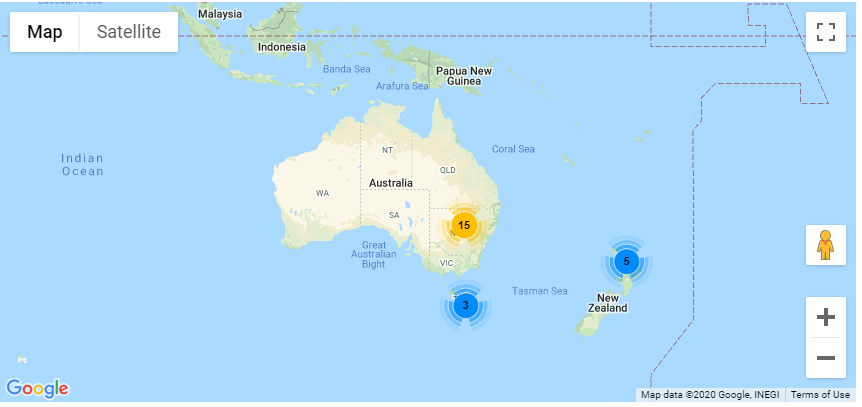
\includegraphics[scale=0.5]{Gambar/marker_clustering.PNG}
	\caption{Contoh Marker Clustering}
	\label{fig:my_label}
\end{figure}
Untuk dapat  menginisialisasi kelas tersebut pihak pengembang perlu menuliskan perintah:
\begin{lstlisting}
    var markerCluster = new MarkerClusterer(map, markers,
            {imagePath: `${path}/m`});
\end{lstlisting}
\textit{Marker Clusterer} sendiri meruapakan suatu library untuk kelas \textit{mark} sehingga kelas ini dapat menggunakan fungsi turunan dari kelas \textit{mark}.

\subsection{HeatMap}
\begin{figure}[H]
	\centering
	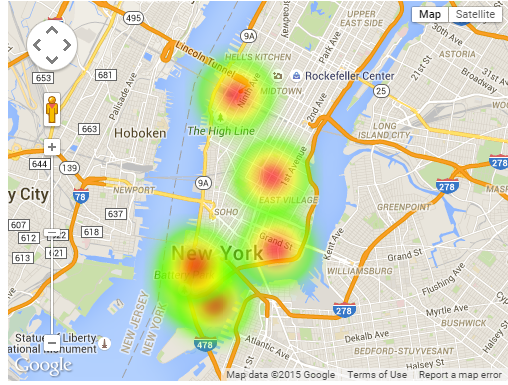
\includegraphics[scale=0.8]{Gambar/heat-map-example.png}
	\caption{Contoh HeatMap}
	\label{fig:my_label}
\end{figure}


\textit{Google Maps Javascript API} telah menyediakan kelas \textit{heatmap} untuk menampilkan \textit{heatmap} pada objek \textit{maps}. Untuk dapat menginisialisasi kelas ini pengembang perlu memanggil perintah \textit{constructor} yang memiliki struktur seperti:
\begin{lstlisting}
    HeatmapLayer([opts])
    Parameters: 
    opts:  HeatmapLayerOptions optional
\end{lstlisting}.

Kelas \textit{HeatMap} dilengkapi dengan parameter \textit{HeatmapLayerOptions} yang bersifat opsional, objek ini  bertujuan untuk dapat mengatur \textit{property} dari kelas \textit{HeatMap}. Parameter \textit{HeatMapLayerOptions} merupakan sebuah objek yang memiliki atribut sebagai berikut:

\begin{itemize}
    \item data \textit{titik-titik} data yang diperlukan.
    \item dissipating variabel yang menentukan apakah \textit{heatmap} akan menghilang jika \textit{maps} diperbesar atau diperkecil.
    \item gardient gardient dari warna \textit{heatmap}
    \item map atribute untuk menunjukan peta dimana \textit{heatmap} akan ditampilkan.
    \item maxIntencity nilai maximal dari intensitas warna pada \textit{heatmap}.
    \item opcity nilai opacity dari \textit{heatmap}.
    \item radius nilai radius dari \textit{heatmap}.
\end{itemize}
Contoh penginisialisasian kelas \textit{heatmap}:
\begin{lstlisting}
    let heatmap = new google.maps.visualization.HeatmapLayer({
            data: heatmapData
        });
\end{lstlisting}
Kelas \textit{HeatMap} memiliki fungsi-fungsi bawaan yang telah disediakan oleh \textit{google maps} beberapa fungsi tersebut adalah:
\begin{itemize}
    \item getData() fungsi ini akan mengembalikan data point pada objek \textit{heatmap}.
    \item getMap() fungsi ini akan mengembalikan objek \textit{map}.
    \item setData(data) fungsi ini akan memasukan data pada objek \textit{heatmap}.
    \item setMap(map) fungsi ini akan memasukan objek \textit{map} pada objek \textit{heatmap}.
    \item setOption(option) fungsi ini akan memasukan  objek \textit{HeatMapLayerOptions} pada objek \textit{heatmap}.
\end{itemize}